\documentclass[a4paper]{article}
\usepackage{graphicx}
\usepackage{amsmath, amsfonts, geometry, float, listings, enumerate, multicol}
\usepackage{multicol, float, color, colortbl}
\usepackage{tikz, titlesec, parskip, pgfplots, filecontents}
\usepackage{hyperref}
\usepackage{amsmath}
\usepackage{tikz, titlesec, parskip}
\usepackage{tikz,pgfplots}
\usepackage[americanvoltages,fulldiodes,siunitx]{circuitikz}
\usetikzlibrary{shapes,arrows}
\usepackage{enumitem}
\titleformat*{\subsubsection}{\LARGE\bfseries}
\usepackage{subcaption}
\usepackage{caption}
\titlespacing{\section}{0pt}{10pt}{0pt}
\titlespacing{\subsection}{0pt}{10pt}{0pt}
\titlespacing{\subsubsection}{0pt}{10pt}{0pt}



\usetikzlibrary{calc,patterns,through}
\newcommand{\arcangle}{%
	\mathord{<\mspace{-9mu}\mathrel{)}\mspace{2mu}}%
}

\renewcommand{\baselinestretch}{1.4}
 \geometry{
 a4paper,
 total={170mm,257mm},
 left=20mm,
 top=20mm,
 }
\usepackage{fancyhdr}
\usepackage{indentfirst}
\pagestyle{fancy}
\fancyhf{}
\rhead{\textbf{پردازش تصاویر دیجیتال}}
\lhead{\textbf{تمرین سری دوم}}
\cfoot{(\space \space \space \space \textbf{\thepage}  \space \space \space)}
\renewcommand{\headrulewidth}{1pt}
\renewcommand{\footrulewidth}{1pt}

 
\usepackage{xepersian}
\setlatintextfont{Times New Roman}
\settextfont{XB Niloofar}
\setdigitfont{XB Niloofar}
\DefaultMathsDigits

\makeatletter
\bidi@patchcmd{\@Abjad}{آ}{الف}
{\typeout{Succeeded in changing آ into الف}}
{\typeout{Failed in changing آ into الف}}
\makeatother
\PersianAlphs

\begin{document}
\begin{minipage}{0.6\textwidth}
\begin{bf}
\begin{center}
	به نام خدا\\
	\vspace{0.25cm}
	دانشگاه صنعتی شریف\\
	\vspace{0.25cm}
	دانشکده مهندسی برق\\
	\vspace{0.5cm}

\large
دکتر عمادالدین فاطمی‌زاده - پردازش تصاویر دیجیتال \\
نیم سال دوم
۱۴۰۱-۱۴۰۰\\
\Large
\vspace{0.4cm}
تمرین عملی سری دوم\\
\end{center}
\end{bf}
\normalsize
\end{minipage} \hfill
\begin{minipage}{0.35\textwidth}
\begin{flushleft}

\includegraphics[width=0.5\textwidth]{Shariflogo.png}\\ \large
\end{flushleft}

 \end{minipage}
\\

\rule[0.1\baselineskip]{\textwidth}{1pt}

\large
\section*{
لطفاً به نکات زیر توجه بفرمایید: (رعایت نکردن این موارد باعث کاهش نمره می‌شود.)
}

\begin{enumerate}
	\item 
نتایج و پاسخ های خود را در یک فایل با فرمت zip به نام
\LR{HW$2$-Name-StudentNumber}
 در سایت  
\href{https://quera.org/course/add_to_course/course/10598/}{\lr{Quera}} 
 قرار دهید. همچنین فایل پایتون یا متلب خود را به همان نام در قسمت مخصوص به خود آپلود کنید.
\item 
کسب نمره کامل در هر سوال مستلزم تحویل  
\textbf{کدها (40 نمره)}
 و
\textbf{توضیحات (30 نمره)}
و
\textbf{نتایج (30 نمره)}
 می‌باشد. 
\item 
کدهای شما تماماً باید توسط خودتان نوشته شده باشند. هرگونه استفاده از کد دیگران، اعم از دوستان و اینترنت، به هر شکل ممکن، تقلب محسوب می‌شود و نمره تمام تمرینات جاری و تمام تمرینات قبلی صفر خواهد شد. با اجرای این کدها باید همان نتایجی که فرستاده اید قابل بازیابی باشند. برنامه شما باید به گونه‌ای باشد که بدون نیاز به هیچ تغییری قابل اجرا باشد، در غیر این‌ صوررت هیچ نمره‌ای تعلق نخواهد گرفت. 
\item 
برای تمام سؤالات، باید جزئیات روشی که استفاده کرده‌اید را توضیح دهید و نتایجی که گرفته‌اید را ارائه دهید. این توضیحات می‌تواند در یک فایل  pdf  و یا در یک فایل  ipynb باشد. در توضیحات، باید اشاره کامل به کارهایی که انجام داده‌اید بنمایید به طوری که یک شخص آگاه از موارد درس بتواند به آسانی متوجه کاری که شما انجام داده‌اید شود.
\item 
در طول ترم امکان ارسال با تاخیر پاسخ  همه‌ی تمارین تا سقف شش روز و در مجموع بیست و یک روز وجود دارد. پس از گذشت این مدت، پاسخ‌های ارسال‌شده پذیرفته نخواهند بود. همچنین، به ازای هر روز تأخیر غیر مجاز  بیست درصد از نمره تمرین به صورت ساعتی کسر خواهد شد.
\item 
 اگر از
\lr{Jupyter notebook} 
 استفاده می‌کنید، میتوانید خروجی‌ها‌ را پاک کنید تا حجم فایل تحویلی زیاد نشود.
\item 
مهلت تحویل: 19 فروردین ساعت 23:59 
\item 
نام طراح هر سوال در زیر آن نوشته شده است و شما میتوانید سوالات خود را از طریق ایمیل یا تلگرام از طراح سوال بپرسید.
\\
محمدامین علم‌الهدی: \lr{Amin@ee.sharif.edu} - \lr{@Alam\_Amin}
\\
سعید رضوی: \lr{Saeedrazavi890@gmail.com} - \lr{@RazooIs}
\\
یاسمین مدقالچی: \lr{Yasmed1379@yahoo.com} - \lr{@Yasssssimed}
\\
صدرا صبوری: \lr{Sadra@ee.sharif.edu} - \lr{@Sadrasabouri}
\\
امیررضا حاتمی‌پور: \lr{Arhp78@gmail.com} - \lr{@Arhp78}
\end{enumerate}
\rule[0.1\baselineskip]{\textwidth}{1pt}

\clearpage
\section*{سوال اول}
\textbf{طراح :‌ سعید رضوی}
\vspace{0.5cm}

در این سوال به دو روش
\lr{sharpen}
 کردن تصاویر در حوزه فرکانس می‌پردازیم. تصویر
\lr{blur} 
 شده اولیه با نام 
\lr{q1.jpg}
را بخوانید.
\begin{enumerate}
	\item 
روش اول: ابتدا نشان دهید که می‌توان تصویر را با استفاده از رابطه
\lr{$F^{-1}{(1+kH_{HP})F}$}
شارپ‌تر کرد که
که $F$ تبدیل فوریه تصویر مورد نظر (بر روی هر کانال دلخواه از تصویر)، $ H_{HP}$ یک فیلتر بالاگذر، و $F^{-1}$ نماد تبدیل فوریه معکوس می‌باشد. (ترجیحا با نوشتن روابط ریاضی رابطه بالا را توجیه کنید، اگر با استفاده از روابط ریاضی موفق نبودید سعی کنید به صورت شهودی آن را توجیه کنید). پس از توجیه این رابطه به پیاده‌سازی آن می‌پردازیم.
 \\
ابتدا تبدیل فوریه‌ تصویر را به دست آورده و اندازه‌ی تبدیل فوریه‌ را نمایش و با نام
\lr{q1\_res01.jpg}
ذخیره کنید.
سپس فیلتر بالاگذر ساخته شده را با نام 
\lr{q1\_res02.jpg}
 ذخیره کنید. سپس خروجی
$ (1+kH_{HP})F$
 را با نام 
\lr{q1\_res03.jpg} 
 ذخیره کنید و آن را با تبدیل فوریه اولیه عکس مقایسه کنید. در نهایت تصویر نهایی را با نام 
\lr{q1\_res04.jpg} 
 ذخیره کنید و ذکر کنید به ازای چه مقدار $ k $ به نتیجه دلخواه خود رسیدید. 
\item
روش دوم: ابتدا نشان دهید که می‌توان تصویر را با استفاده از رابطه 
$f + kF^{-1}\{4\pi^2(u^2+v^2)F(u,v)\}$
 که 
$ f $
 عکس ورودی در حوزه‌ی زمان،
$F(u,v)$ 
 تبدیل فوریه تصویر مورد نظر (بر روی هر کانال دلخواه از تصویر)، 
$(u ,v)$
  متغیر های فوریه در حوزه فرکانس می‌باشد (هم ارز $(x,y)$ در حوزه مکان) و 
$F^{-1}$
 نماد تبدیل فوریه معکوس می‌باشد، شارپ‌تر کرد (ترجیحا با نوشتن روابط ریاضی رابطه بالا را توجیه کنید، اگر با استفاده از روابط ریاضی موفق نبودید سعی کنید به صورت شهودی آن را توجیه کنید). حال به پیاده سازی رابطه بالا می پردازیم :
اندازه 
$ 4\pi^2(u^2+v^2)F(u,v) $ 
را نمایش دهید و با نام 
\lr{q1\_res05.jpg}
 ذخیره کنید. 
 سپس
$F^{-1}\{4\pi^2(u^2+v^2)F(u,v)\}$
 را که همان
\lr{unsharp mask} 
ما می‌باشد را با نام  
\lr{q1\_res06.jpg}
ذخیره کنید. در نهایت تصویر نهایی را با نام  
\lr{q1\_res07.jp} 
ذخیره کنید و ذکر کنید به ازای چه مقدار $k$ به نتیجه دلخواه خود رسیدید.
\end{enumerate}


\section*{سوال دوم}
\textbf{طراح : سعید رضوی }
\vspace{0.3cm}

در این سوال قصد داریم با استفاده از روش
 \lr{Laplacian stack} 
(پشته لاپلاسین) به ترکیب دو عکس به صورتی بپردازیم که نتیجه حاصل بسیار طبیعی باشد. در ادامه این روش  را توضیح می‌دهیم. برای به دست‌آوردن پشته‌ی ‌لاپلاسین نیازمند به آشنایی با
 \lr{Gaussian stack} 
(پشته‌ی گاوسی) هستیم. 
تعریف پشته‌ی گاوسی با $ n $ سطح
\lr{(level)}
برابر است با مجموعه ی $ n $ تصویر
\lr{blur}
 شده از یک تصویر مشخص که در هر مرحله بالاتر، تصویر با شدت بیشتری 
\lr{blur}
  شده‌است. (اگر بخواهیم تفسیری از پشته های گاوسی در حوزه زمان داشته باشیم، مثل این است که در هر مرحله تصویر را با یک فیلتر گوسی با انحراف معیار بیشتری کانوالو کرده و در نتیجه هر مرحله که بالاتر میرویم، پشته گاوسی ما تصویری محو‌تر از تصویر اصلی است) نمونه‌ای از پشته‌های گاوسی را برای یک تصویر دلخواه در‌شکل زیر مشاهده می‌کنید:
\begin{figure}[H]
	\centering
	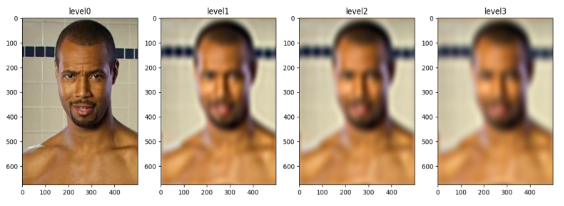
\includegraphics[width=0.6 \linewidth]{images/Picture1.png}
\end{figure}
دقت شود در این سوال
\lr{blur}
کردن تصاویر و ساخت پشته‌های گاوسی باید در حوزه فرکانس انجام شود و مجاز به کانوالو کردن تصاویر با فیلتر گوسی در حوزه زمان نیستید. اما در ادامه می‌توانید پس از
\lr{blur} 
کردن در حوزه فرکانس آن را به حوزه مکان برگردانید و ادامه‌ی کار را در حوزه مکان انجام دهید .
حال به تعریف
 \lr{Laplacian stack} 
(پشته لاپلاسین) می‌پردازیم: لاپلاسین پشته در مرحله $ i $ ام از رابطه زیر به دست می‌آید: 
\begin{equation*}
	l_{s_i}=G_{s_i}-G_{s_{i+1}}
\end{equation*}
که$ G_{s_i}$ پشته‌ی ‌گاوسی تصویر در مرحله $ i $ام می باشد. همانطور که می‌توانید حدس بزنید پشته‌لاپلاسین دارای جزئیات تصویر در هر مرحله است. نکته مهمی که باید به آن توجه داشت این است که پشته‌ی ‌لاپلاسین در مرحله آخر همان پشته‌ی ‌گاوسی در مرحله آخر است یعنی
 $l_{s_{\ last\ level}}=G_{s_{\ last\ level}}$ 
 (توجیه کنید دلیل برابری پشته‌ی ‌لاپلاسین و پشته‌ی ‌گاوسی در مرحله آخر چیست و چه کمکی به ترکیب تصاویر می‌کند؟).
نکته مهم دیگر در ترکیب دو تصویر این است که برای این که مشخص کنیم چه بخشی از تصویر نهایی از تصویر اول و چه بخشی از تصویر نهایی از تصویر دوم تشکیل شده باید یک ماسک باینری
 \lr{(binary mask)} 
 مشخص کنیم (این ماسک باینری که یک ماسک سیاه و سفید است مشخص میکند که برای مثال ناحیه سفید رنگ تصویر باید از تصویر اول بیاید و ناحیه سیاه رنگ تصویر از تصویر دوم). در انتها پس از به دست آوردن پشته‌های‌لاپلاسین باید آن‌ها را در هر مرحله به صورت مناسب با یکدیگر جمع کرده. جمع پشته‌لاپلاسین دو عکس در هر مرحله از رابطه زیر بدست می‌آید‌: 
\begin{equation*}
	l_{s_i\ blended\ image}=l_{s_i\ image1}G_{s_i\ mask\ }+l_{s_i\ image2}{(1-G}_{s_i\ mask\ })
\end{equation*}
در رابطه بالا
 $G_{s_i\ mask}$ 
پشته‌ی ‌گاوسی مرحله $ i $‌ام ماسک می‌باشد. پس از تشکیل شدن پشته‌‌های لاپلاسین تصویر نهایی با جمع کردن تمام آنها با یکدیگر باید به جواب نهایی و تصویر ترکیب شده خود برسید. نمونه‌ای از ترکیب دو عکس با استفاده از این روش در ادامه آمده است. برای این سوال شما هم دو تصویر به دلخواه خودتان انتخاب کنید و با توضیحات بالا آن دو را به صورت دلخواه با هم ترکیب کنید.
\lr{
	\begin{figure}[H]
		\centering
		\begin{subfigure}[b]{0.2\linewidth}
			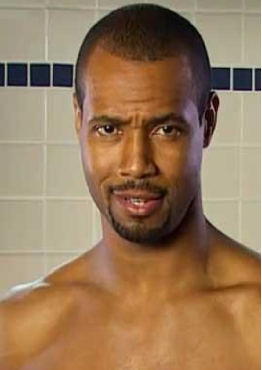
\includegraphics[width=\linewidth]{images/Picture2.png}
			\caption*{Image I}
		\end{subfigure}
		\begin{subfigure}[b]{0.2\linewidth}
			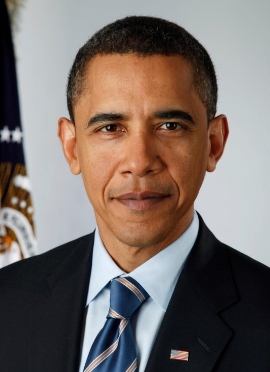
\includegraphics[width=\linewidth]{images/Picture3.png}
			\caption*{Image II}
		\end{subfigure}
		\begin{subfigure}[b]{0.2\linewidth}
			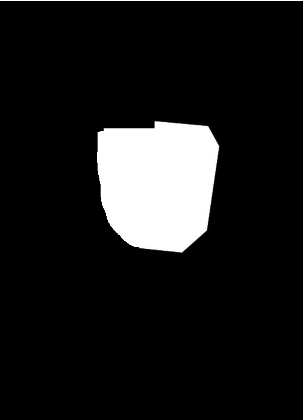
\includegraphics[width=\linewidth]{images/Picture4.png}
			\caption*{Mask}
		\end{subfigure}
		\begin{subfigure}[b]{0.2\linewidth}
			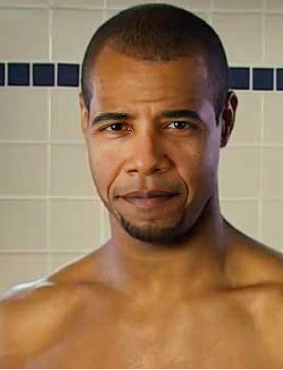
\includegraphics[width=\linewidth]{images/Picture5.png}
			\caption*{Blended Image}
		\end{subfigure}
	\end{figure}
}
برای ساختن ماسک می‌توانید از هر نرم افزار دلخواهی مثل 
\lr{Paint},
\lr{Photoshop}
استفاده کنید.
\section*{سوال سوم}
\textbf{طراح :‌ یاسمین مدقالچی }
\vspace{0.3cm}

در این سوال می‌خواهیم با  عملکرد و نحوه‌ی پیاده سازی مدل‌های مختلف الگوریتم
\lr{retinex}
 آشنا شویم. هم چنین می‌خواهیم این پیاده سازی‌ها بر اساس مقاله 
\href{https://www.ipol.im/pub/art/2014/107/article.pdf}{\lr{Multi Scale Retinex}} 
که در پوشه‌ی درس قرار گرفته شده است انجام شود.
\begin{enumerate}
\item 
عکس \lr{q3.jpeg} را \lr{load} کرده و نمایش دهید.
\item 
ابتدا قسمت
$  2.1  $
مقاله 
\lr{(Single scale Retinex)} 
را مطالعه کرده و به صورت مختصر در گزارش کار خود آن را توضیح دهید. الگوریتم
\lr{SSR} 
 را به عنوان تابعی با همین نام پیاده کنید  و عملکرد این تابع را بر روی عکس
\lr{load} 
 شده بسنجید و خروجی تولید شده را در گزارش کار خود قرار دهید.
\item 
قسمت
$ 2.2  $
مقاله
\lr{(Multi scale Retinex)} 
را مطالعه کرده و تفاوت آن با قسمت قبل را توضیح دهید و هم چنین الگوریتم را در قالب تابعی به نام
 \lr{MSR}
 پیاده کنید و عملکرد این تابع را بر روی عکس
 \lr{load} 
شده بسنجید و خروجی آن را در گزارش خود بیاورید. 
\item 
الگوریتم
 \lr{MSRCR}
  را در قسمت
$  2.3 $
 مقاله مطالعه کرده و در مورد فرق‌های آن با
\lr{SSR} 
 توضیح دهید و مانند قسمت‌های قبل آن را در قالب یک تابع پیاده کنید و نتایج را در گزارش خود بیاورید.
\item 
الگوریتم
 \lr{MSRCP} 
را نیز پیاده کنید و نتایج را در گزارش کار خود بیاورید.
\end{enumerate}

\section*{سوال چهارم}
\textbf{طراح :‌ امیررضا حاتمی‌پور}
\vspace{0.3cm}

\begin{enumerate}
	\item 
هر کدام از روش های
\lr{HE}
\RTLfootnote{\lr{Histogram equalization}}
, 
\lr{AHE} 
\RTLfootnote{\lr{Adaptive histogram equalization}} , 
\lr{CLAHE}
\RTLfootnote{\lr{Contrast limited adaptive histogram equalization}}
را توضیح دهید. سپس فرض کنید تصویر ورودی به شکل زیر باشد.
\begin{figure}[H]
	\centering
	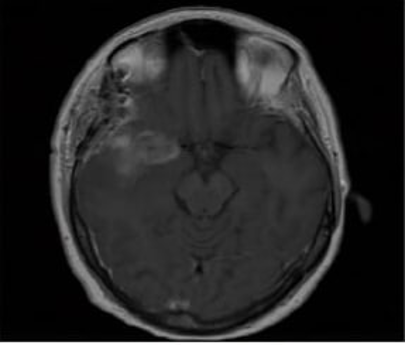
\includegraphics[width=0.3 \linewidth]{images/Picture6.png}
\end{figure}
حال مشخص کنید که خروجی‌های زیر هر کدام برای کدام یک از این سه روش است.
\lr{
	\begin{figure}[H]
		\centering
		\begin{subfigure}[b]{0.3\linewidth}
			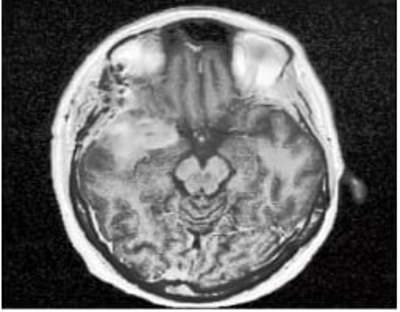
\includegraphics[width=\linewidth]{images/Picture7.png}
			\caption*{Image I}
		\end{subfigure}
		\begin{subfigure}[b]{0.3\linewidth}
			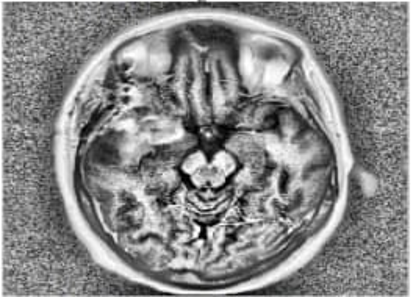
\includegraphics[width=\linewidth]{images/Picture8.png}
			\caption*{Image II}
		\end{subfigure}
	\end{figure}
}
\item
برای تصویر
\lr{q4.png} 
روش های HE، AHE و CLAHE را پیاده کنید و خروجی‌ها را در فایل 
\lr{q4\_1.png}، 
\lr{q4\_2.png}
 و
\lr{q4\_3.png}
   ذخیره کنید.
\end{enumerate}

\section*{سوال پنجم}
\textbf{طراح :‌ صدرا صبوری}
\vspace{0.3cm}

\href{https://en.wikipedia.org/wiki/Zone_plate}{صفحه‌ی منطقه‌ای }
تصویری از مجموعه دوایر هم‌مرکز است که یک در میان تغییر رنگ می‌دهند. در واقع در این تصویر فرکانس‌های مختلف در شعاع‌های متفاوت دیده می‌شوند. نمونه‌ای از این فایل به نام 
\lr{q5.png}
در اختیار شما قرار گرفته‌است. با توجه به سوالات زیر پاسخ دهید.
\begin{enumerate}
	\item

به ترتیب فیلترهای 
\href{https://en.wikipedia.org/wiki/Sobel_operator}{سوبل} 
و گوسی و لاپلاسین (با مقادیر دلخواه) اعمال کنید و نتایج را در
 \lr{q5\_res01.png}
 و
  \lr{q5\_res02.png} 
 و
  \lr{q5\_res03.png} 
 ذخیره کنید و تفاوت‌ها و شباهت‌های آن‌ها را بیان کنید.

\item
ابتدا نشان دهید که تبدیل فوریه یک فیلتر گوسی همچنان گوسی است. سپس تصویر اولیه را به حوزه فرکانس ببرید و تصویر متقارن شده آن را در مقیاس لگاریتمی در حوزه فرکانس نمایش دهید و با نام  
\lr{q5\_res04.png} 
ذخیره کنید. 
\\
حال با ضرب کردن فیلتر گوسی (معادل فرکانسی فیلتر گوسی قسمت قبل) در تبدیل فوریه تصویر تصویر 
\lr{q5\_res05.png}
 را ذخیره کنید و سپس با ضرب 
\href{https://en.wikipedia.org/wiki/Negative_(photography)}{متمم}
این فیلتر تصویر
 \lr{q5\_res06.png}
 را ذخیره کنید. هر دوی این تصاویر را از حوزه فرکانس برگردانید و نام تصاویر ایجاد شده را به ترتیب
 \lr{q5\_res07.png} 
و 
\lr{q5\_res08.png} 
بنامید.
همین مراحل را برای یک فیلتر مربعی در حوزه‌ی فرکانس انجام دهید و تصاویر را به ترتیب 
\lr{q5\_res09.png} 
و 
\lr{q5\_res10.png} 
و 
\lr{q5\_res11.png} 
و 
\lr{q5\_res12.png}
بنامیم.
خروجی ها را با هم مقایسه کنید. علت به وجود آمدن مربع‌های کوچک در تصاویری که از فیلتر مربعی گذشتند چیست؟
\item
یک بار تصویر اولیه را با بزرگ‌نمایی ذخیره کنید (نام آن را 
\lr{q5\_res13.png})
 و یکبار با کوچک نمایی (نام آن را 
 \lr{q5\_res14.png})
  قرار دهید و مشابهت هر کدام از آن‌ها را با نتایج قسمت‌های قبل مقایسه کنید و دلیل این مشابهت را بیان کنید.
\end{enumerate}
\section*{سوال ششم }
\textbf{طراح :‌ محمدامین علم‌الهدی }
\vspace{0.3cm}
\\
در این سوال قصد داریم با استفاده از روش
 \lr{template matching}،
 حرف
  \lr{B} 
 را از بین حروف دیگر الفبای انگلیسی تشخیص دهیم. برای ادامه‌ی تمرین، از دو تصویر زیر که به ترتیب در فایل های 
 \lr{q7\_1.png} 
 و
  \lr{q7\_2.png} 
 آمده‌اند استفاده کنید.
\lr{
	\begin{figure}[h!]
		\centering
		\begin{subfigure}[b]{0.91\linewidth}
			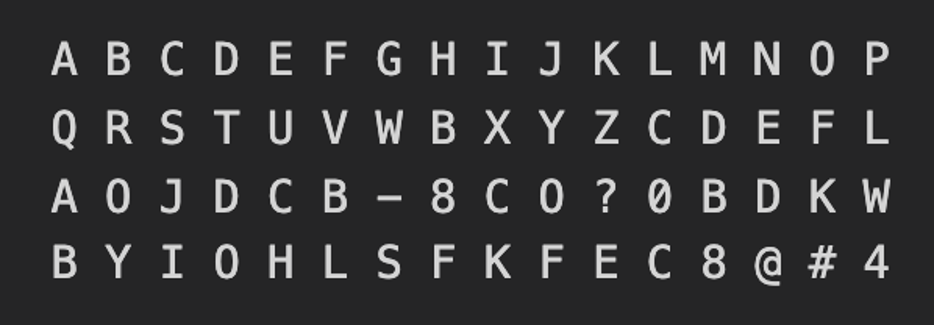
\includegraphics[width=\linewidth]{images/Picture13.png}
		\end{subfigure}
		\begin{subfigure}[b]{0.1\linewidth}
			
\includegraphics[width=\linewidth]{images/Picture14.png}
		\end{subfigure}
	\end{figure}
}
برای آشنایی بیشتر با انواع روش‌های مختلف
 \lr{temple matching} 
میتوانید از 
\href{https://docs.adaptive-vision.com/4.7/studio/machine_vision_guide/TemplateMatching.html}{این لینک}
استفاده کنید. ۲ روش از روش‌های ذکر شده در لینک قبل را بر روی تصویر اعمال کنید و نتیجه‌ی آن به همراه توضیح روش انجام تمامی مراحل را در گزارش کار خود ذکر کنید. در صورتی که روش‌ انتخابی شما به نتیجه‌ی مطلوب نرسید، سعی کنید دلیل آن را توضیح دهید.
\section*{ سوال هفتم - امتیازی (۱۵ نمره از ۱۰۰ نمره)}
\textbf{طراح :‌ محمدامین علم‌الهدی }
\vspace{0.3cm}

در این سوال قصد داریم به کمک فیلترهای پایین گذر و بالا گذر، یک تصویر هیبریدی بسازیم. تصویر هیبریدی به تصویری گفته می‌شود که وقتی از نزدیک به آن نگاه می‌کنیم یک تصویر، و وقتی از دور به آن نگاه می‌کنیم تصویر دیگری می‌بینیم. به طور مثال، تصویر زیر یک تصویر هیبریدی است. هنگامی که از نزدیک به آن نگاه می کنید تصویر انیشتین را می بینید و وقتی از فاصله دورتر به آن نگاه کنید، تصویر دیگری را خواهید دید.
\begin{figure}[h]
	\centering
	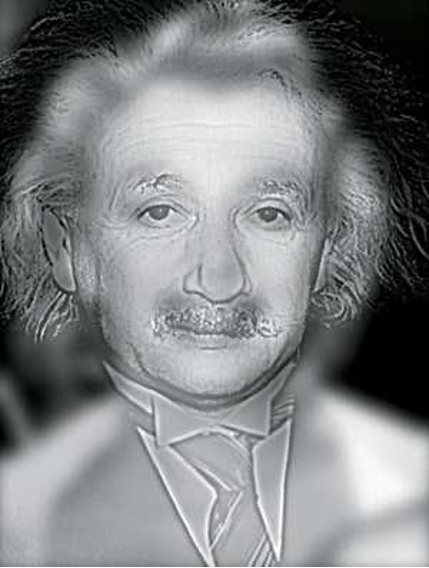
\includegraphics[width=0.3 \linewidth]{images/Picture9.png}
\end{figure}
در ادامه نمونه یکی از این تصاویر را می بینید. شما می‌توانید به دلخواه دو تصویر انتخاب کنید. مطالعه \href{https://stanford.edu/class/ee367/reading/OlivaTorralb_Hybrid_Siggraph06.pdf}{این مقاله}
برای رسیدن به نتایج بهتر در این قسمت توصیه می‌شود.
\lr{
	\begin{figure}[H]
		\centering
		\begin{subfigure}[b]{0.3\linewidth}
			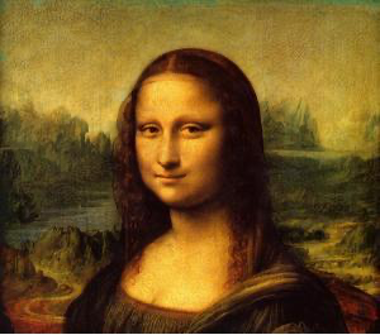
\includegraphics[width=\linewidth]{images/Picture10.png}
		\end{subfigure}
		\begin{subfigure}[b]{0.3\linewidth}
			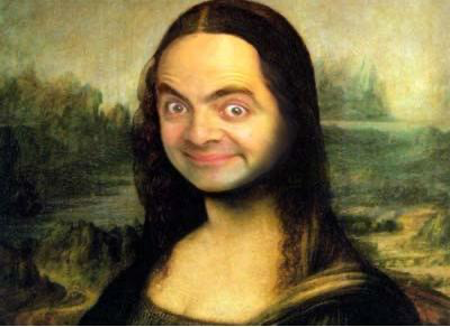
\includegraphics[width=\linewidth]{images/Picture11.png}
		\end{subfigure}
	\end{figure}
}
برای به دست آوردن نتیجه بهتر، باید دو تصویر را هم اندازه کرده و با هم منطبق نمایید، یعنی قسمت‌های مشابه یا معادل را روی هم قرار دهید. برای مثال، اگر بخواهید دو تصویر از صورت دو شخص را باهم ادغام کنید، بهتر است در ابتدا دو تصویر را طوری تغییر دهید تا اجزای متناظر صورت دو شخص در یک مکان از تصویرشان قرارگیرد. می توانید این کار را با تطبیق چشم‌ها انجام دهید. چون شکل کلی صورت انسان ها یکسان می‌باشد، اگر چشم‌ها منطبق شده باشند می‌توان انتظار داشت که با تقریب نسبتا خوبی بقیه قسمت‌ها نیز با هم منطبق شده‌اند. این کار را می‌توانید با انتخاب چند نقطه متناظر بین دو تصویر و استفاده از نگاشت‌های هندسی فضای دو بعدی (چرخش و انتقال) انجام دهید. اینکار را باید خودتان انجام دهید و نمی‌توانید از کدهای موجود در اینترنت استفاده نمایید. همچنین از انجام برخی پیش پردازش‌ها بر روی تصاویر مثل نرمالایز کردن و تبدیل
 \lr{RGB} 
به 
\lr{Grayscale}
غافل نشوید. توجه کنید که سایز دو تصویر نیز باید یکسان باشد، پس بعد از اینکه دو تصویر بر روی یکدیگر 
 \lr{register}
شدند، سایز هر دو را یکی کنید.

هنگامی که از فاصله‌ی نزدیک به یک تصویر نگاه کنیم بیشتر جزئيات آن تصویر را میبینیم. علت این است که بیشتر جزئیات کوچک تصاویر در فرکانس‌های بالا ذخیره شده‌اند و جزئیات کلی تصویر در فرکانس‌های پایین ذخیره شده‌اند. بنابراین در تصویری که میخواهید از نزدیک دیده شود باید فرکانس‌های پایین را حذف کرده و فرکانس‌های بالا را نگه دارید (و بالعکس برای تصویری که می‌خواهید وقتی از دور به آن نگاه می‌کنید دیده شود). برای انجام این کار، ابتدا نیاز داریم که دو تصویر را به حوزه‌ی فرکانس ببریم. اینکار را میتوانید توسط توابع آماده‌ یا با استفاده از فرمول تبدیل فوریه $ 2 $ بعدی انجام دهید. در مرحله‌ی بعد باید با استفاده از فیلتر‌های پایین گذر و بالا گذر، تصاویر را فیلتر کنیم. برای فیلتر، از فیلتر گوسی دو بعدی استفاده کنید (پارامتر‌های فیلتر مانند فرکانس
\lr{cutoff}
و انحراف از معیار را خودتان انتخاب کنید و حتما در گزارش کار ذکر کنید). می‌توانید مقدار 
\lr{cutoff}
 را برای هر دو فیلتر بالاگذر و پایین گذر یکسان در نظر بگیرید ولی برای کسب بهترین نتیجه، باید این دو مقدار را متفاوت در نظر بگیرید به طوری که
  \lr{cutoff}
   برای فیلتر بالاگذر کوچک‌تر از مقدار برای فیلتر پایین گذر باشد. در اینصورت هر دو تصویر در دامنه فرکانس در یک نوار مشترک غیر صفر می‌شوند. برای ترکیب دو تصویر در این نوار، از میانگین‌گیری وزن‌دار استفاده نمایید (به محتوای فرکانسی هر تصویر یک ضریب اختصاص دهید و با هم در حوزه فرکانس جمعشان کنید).
تصویر خروجی در مثال گفته شده به صورت زیر می‌باشد:
\begin{figure}[H]
	\centering
	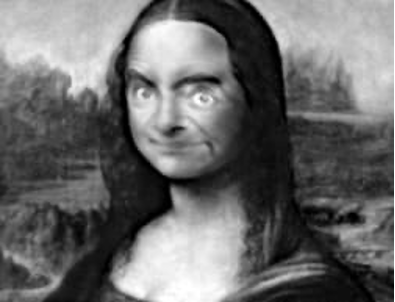
\includegraphics[width=0.3 \linewidth]{images/Picture12.png}
\end{figure}
\newpage
لطفا تمامی مراحل کار خود را به صورت کامل در گزارش کار توضیح دهید و سعی کنید عکس‌هایی که در گزارش کار قرار میدهید، \lr{caption} مناسب داشته باشند. همچنین فایل تصاویر خواسته شده در ادامه را داخل فایل تحویلی خود با نام گذاری مناسب قرار دهید:
۱- عکس هر دو تصویر بعد از اعمال نگاشت‌ها و یکسان شدن سایز‌ ۲- هر دو تصویر در حوزه‌ی فرکانس قبل از اعمال فیلتر ۳- تصویر‌های فیلتر شده در حوزه‌ی فرکانس ۴- تصویر هیبرید نهایی

\end{document}
